\documentclass[11pt]{article}

% --- PAQUETS ESSENTIELS ---
\usepackage{acl}
\usepackage{times}
\usepackage{latexsym}
\usepackage{booktabs}
\usepackage[T1]{fontenc}
\usepackage[utf8]{inputenc}
\usepackage[french]{babel}
\usepackage{enumitem}
\usepackage{graphicx}
\usepackage{hyperref}
\hypersetup{
    colorlinks=true,
    linkcolor=blue,
    urlcolor=blue,
    citecolor=blue
}
\usepackage{url}
\usepackage{multirow}

\title{Analyse Statistique et Sémantique des Discours Présidentiels Sud-Coréens (1948-2022)}

\author{
Marcel Nguyen \\
\texttt{marcel.nguyen@gmail.com} \\
}

\begin{document}
\maketitle

\begin{abstract}
Cet article présente une analyse textométrique et thématique exhaustive du corpus des discours présidentiels de la Corée du Sud, couvrant la période de 1948 à 2022. À travers l'utilisation d'outils de textométrie (TXM) et de modèles de thématiques latentes (LDA, LSA), nous explorons l'évolution du lexique politique sur douze mandats présidentiels. Nous mettons en évidence une stabilité remarquable du vocabulaire institutionnel contrastant avec des ruptures thématiques fortes liées aux crises historiques et sanitaires. Nos résultats montrent que si des termes comme \textit{Gouvernement} ou \textit{Nécessité} constituent le socle invariant du discours, des signatures spécifiques comme la \textit{Crise du FMI} ou la pandémie de \textit{COVID-19} permettent une classification précise des périodes politiques.
\end{abstract}

\section*{Mots-clés}
Analyse de discours ; Textométrie ; Coréen ; LDA ; Spécificité de Lafon ; Corée du Sud.

\section{Introduction}
Le discours présidentiel en Corée du Sud constitue un observatoire privilégié des mutations idéologiques et sociales d'une nation passée d'un régime autoritaire à une démocratie libérale en quelques décennies. L'analyse automatique de ce corpus massif (plus de 9 000 discours) nécessite des méthodes robustes capables de gérer les spécificités morphologiques du coréen. Cet article détaille une méthodologie hybride alliant la textométrie classique, basée sur les indices de spécificité, et le \textit{topic modeling} via l'Allocation de Dirichlet Latente (LDA) et l'Analyse Sémantique Latente (LSA).

\section{Données et Prétraitement}
\subsection{Description et Constitution du Corpus}
Les données utilisées dans cette étude proviennent des Archives Présidentielles de la République de Corée. Ce corpus unique couvre douze présidences, de la fondation de la République sous Lee Seung-man (1948) jusqu'à la fin du mandat de Moon Jae-in (2022). 

Le corpus se compose de 9 984 documents pour un total de 345 491 paragraphes. On observe une croissance exponentielle de la production discursive au fil des décennies, reflétant une institutionnalisation accrue de la communication politique. À titre d'exemple, le président Park Chung-hee totalise 1 324 discours sur 18 ans, tandis que Moon Jae-in en produit 1 392 en seulement 5 ans. Cette densité textuelle moderne offre un défi de traitement particulier.

\subsection{Évaluation des Analyseurs Morphosyntaxiques}
Le coréen étant une langue agglutinante, le "mot" graphique (eojeol) n'est pas l'unité sémantique de base. Une phase de lemmatisation et de segmentation en morphèmes est impérative. Nous avons évalué trois outils de la suite \texttt{KoNLPy} :
\begin{itemize}
    \item \textbf{Hannanum} : Performant pour le texte général mais moins précis sur les termes techniques.
    \item \textbf{Komoran} : Excellent pour le traitement de masse (débit de 15,4 discours/sec), utilisé pour les phases de prétraitement rapide.
    \item \textbf{Kkma} : Analyseur très précis mais lent (débit de 1,9 discours/sec). C'est cet outil que nous avons privilégié pour la génération du corpus XML-TEI final, car sa finesse d'étiquetage permet de distinguer précisément les noms communs (étiquette \texttt{NNG}) des noms propres (\texttt{NNP}), évitant ainsi des ambiguïtés majeures dans le calcul des spécificités.
\end{itemize}

\section{Analyse Textométrique (TXM)}
L'approche textométrique s'appuie sur une structure de données XML où chaque texte est enrichi de métadonnées (président, date, titre).

\subsection{Indice de Spécificité de Lafon}
L'outil central de notre analyse est l'indice de spécificité, qui mesure l'écart entre la fréquence observée d'un terme dans un sous-corpus (un président) et sa fréquence attendue si la distribution était aléatoire dans le corpus total.
Le calcul repose sur la loi hypergéométrique :
\[ P(X \ge f) = \sum_{i=f}^{n} \frac{\binom{t}{i} \binom{N-t}{n-i}}{\binom{N}{n}} \]
où $N$ est la taille du corpus total, $n$ la taille du sous-corpus, $t$ la fréquence totale du mot et $f$ sa fréquence observée.

\subsection{Analyse des Signatures Thématiques}
Les résultats (Tableau \ref{tab:signatures_complete}) montrent une polarisation thématique forte.
\begin{itemize}
    \item \textbf{Moon Jae-in} : Sa signature est dominée par la gestion de crise (\textit{Corona}, \textit{Vaccin}, \textit{Quarantaine}) avec des scores de spécificité dépassant 1400, illustrant une absorption quasi totale du discours par l'urgence sanitaire.
    \item \textbf{Park Geun-hye} : Un vocabulaire orienté vers la modernité économique (\textit{Économie Créative}, \textit{Innovation}, \textit{Start-up}).
    \item \textbf{Kim Dae-jung} : Son mandat est marqué par deux piliers : la réponse à la crise financière de 1997 (\textit{FMI}, \textit{Devises}) et la politique de rapprochement avec le Nord (\textit{Sunshine Policy}).
    \item \textbf{Park Chung-hee} : Une rhétorique de construction nationale physique (\textit{Modernisation}, \textit{Industrie}, \textit{Rural}, \textit{Construction}).
\end{itemize}

\begin{table}[t]
\centering
\small
\begin{tabular}{llc}
\toprule
\textbf{Président} & \textbf{Terme dominant} & \textbf{Indice} \\
\midrule
Moon Jae-in & Corona (코로나) & 1486.4 \\
Lee Seung-man & Peuple/Homme (사람) & 1638.1 \\
Park Chung-hee & Modernisation (근대화) & 854.4 \\
Kim Dae-jung & Devises (외환) & 680.2 \\
Lee Myung-bak & Croissance Verte (녹색) & 714.9 \\
\bottomrule
\end{tabular}
\caption{Principales signatures lexicales (Indices de Lafon).}
\label{tab:signatures_complete}
\end{table}

\subsection{Stabilité et Invariants Lexicaux}
Une analyse par Coefficient de Variation (CV) a permis de dégager les termes les plus stables. Le terme \textbf{Besoin} (\textit{pillyo}) est le plus constant à travers 70 ans d'histoire, suivi de \textbf{Gouvernement} (\textit{jeongbu}). Cette stabilité suggère un "socle institutionnel" immuable, quel que soit le bord politique de l'orateur. À l'inverse, les points de divergence maximale (variance élevée) correspondent aux noms de crises ou de programmes politiques spécifiques.

\section{Modélisation Thématique (LDA/LSA)}
Pour compléter l'approche lexicale, nous avons utilisé des modèles probabilistes pour extraire les thématiques latentes indépendantes des choix de mots spécifiques.

\subsection{Résultats de l'Allocation de Dirichlet Latente (LDA)}
Le modèle LDA (15 thèmes) a identifié des clusters sémantiques cohérents. Le Thème 11 (\textit{Relations Internationales}) regroupe les termes \textit{Monde}, \textit{Asie}, \textit{Corée}, illustrant une préoccupation constante pour l'insertion mondiale. Le Thème 13 (\textit{Sécurité et Nord}) se focalise sur les relations inter-coréennes, montrant une persistance thématique forte malgré les changements de présidence.

\subsection{Comparaison LSA vs LDA}
L'Analyse Sémantique Latente (LSA) a été testée en parallèle. Alors que LDA offre une meilleure interprétabilité des thèmes "humains", LSA s'est avérée plus efficace pour identifier les structures de co-occurrence de haut niveau à travers les paragraphes courts. L'utilisation de GPU via PyTorch a réduit le temps de traitement de 40\% par rapport aux implémentations CPU classiques (scikit-learn).

\section{Discussion}
L'hybridation des méthodes TXM et LDA apporte une vision bi-dimensionnelle du discours. TXM excelle dans l'identification des ruptures (ce qui rend un président unique), tandis que LDA capture les continuités thématiques (ce sur quoi tout le monde parle). L'analyse montre que le discours politique coréen s'est "professionnalisé" : le vocabulaire est passé de termes très émotionnels et patriotiques sous Lee Seung-man à un vocabulaire technique d'expert-comptable ou de gestionnaire de crise à partir des années 2000.

\section{Conclusion}
Cette recherche valide l'efficacité des chaînes de traitement TAL sur le coréen pour l'analyse diachronique de longue durée. Le passage par un format XML normé pour TXM assure une pérennité des données et permet des allers-retours entre statistiques globales et lecture fine (concordances). Les futurs travaux pourraient explorer l'évolution du sentiment associé à ces thématiques pour nuancer la compréhension de la rhétorique politique sud-coréenne.

\bibliographystyle{acl_natbib}
\begin{thebibliography}{10}
\bibitem{lafon1980} Lafon, P. (1980). Sur la variabilité de la fréquence des formes dans un corpus. \textit{Mots}, 1(1), 127-165.
\bibitem{blei2003} Blei, D. M., et al. (2003). Latent Dirichlet allocation. \textit{Journal of Machine Learning Research}.
\bibitem{forest2009} Forest, D., et al. (2009). Identification automatique du parti politique : une approche lexicométrique. \textit{DEFT 2009}.
\bibitem{konlpy2014} Park, E. L., et al. (2014). KoNLPy: Korean natural language processing in Python. \textit{ACL 2014}.
\end{thebibliography}

\clearpage
\onecolumn
\appendix
\section{Annexes : Visualisations Thématiques}

\begin{figure}[h]
    \centering
    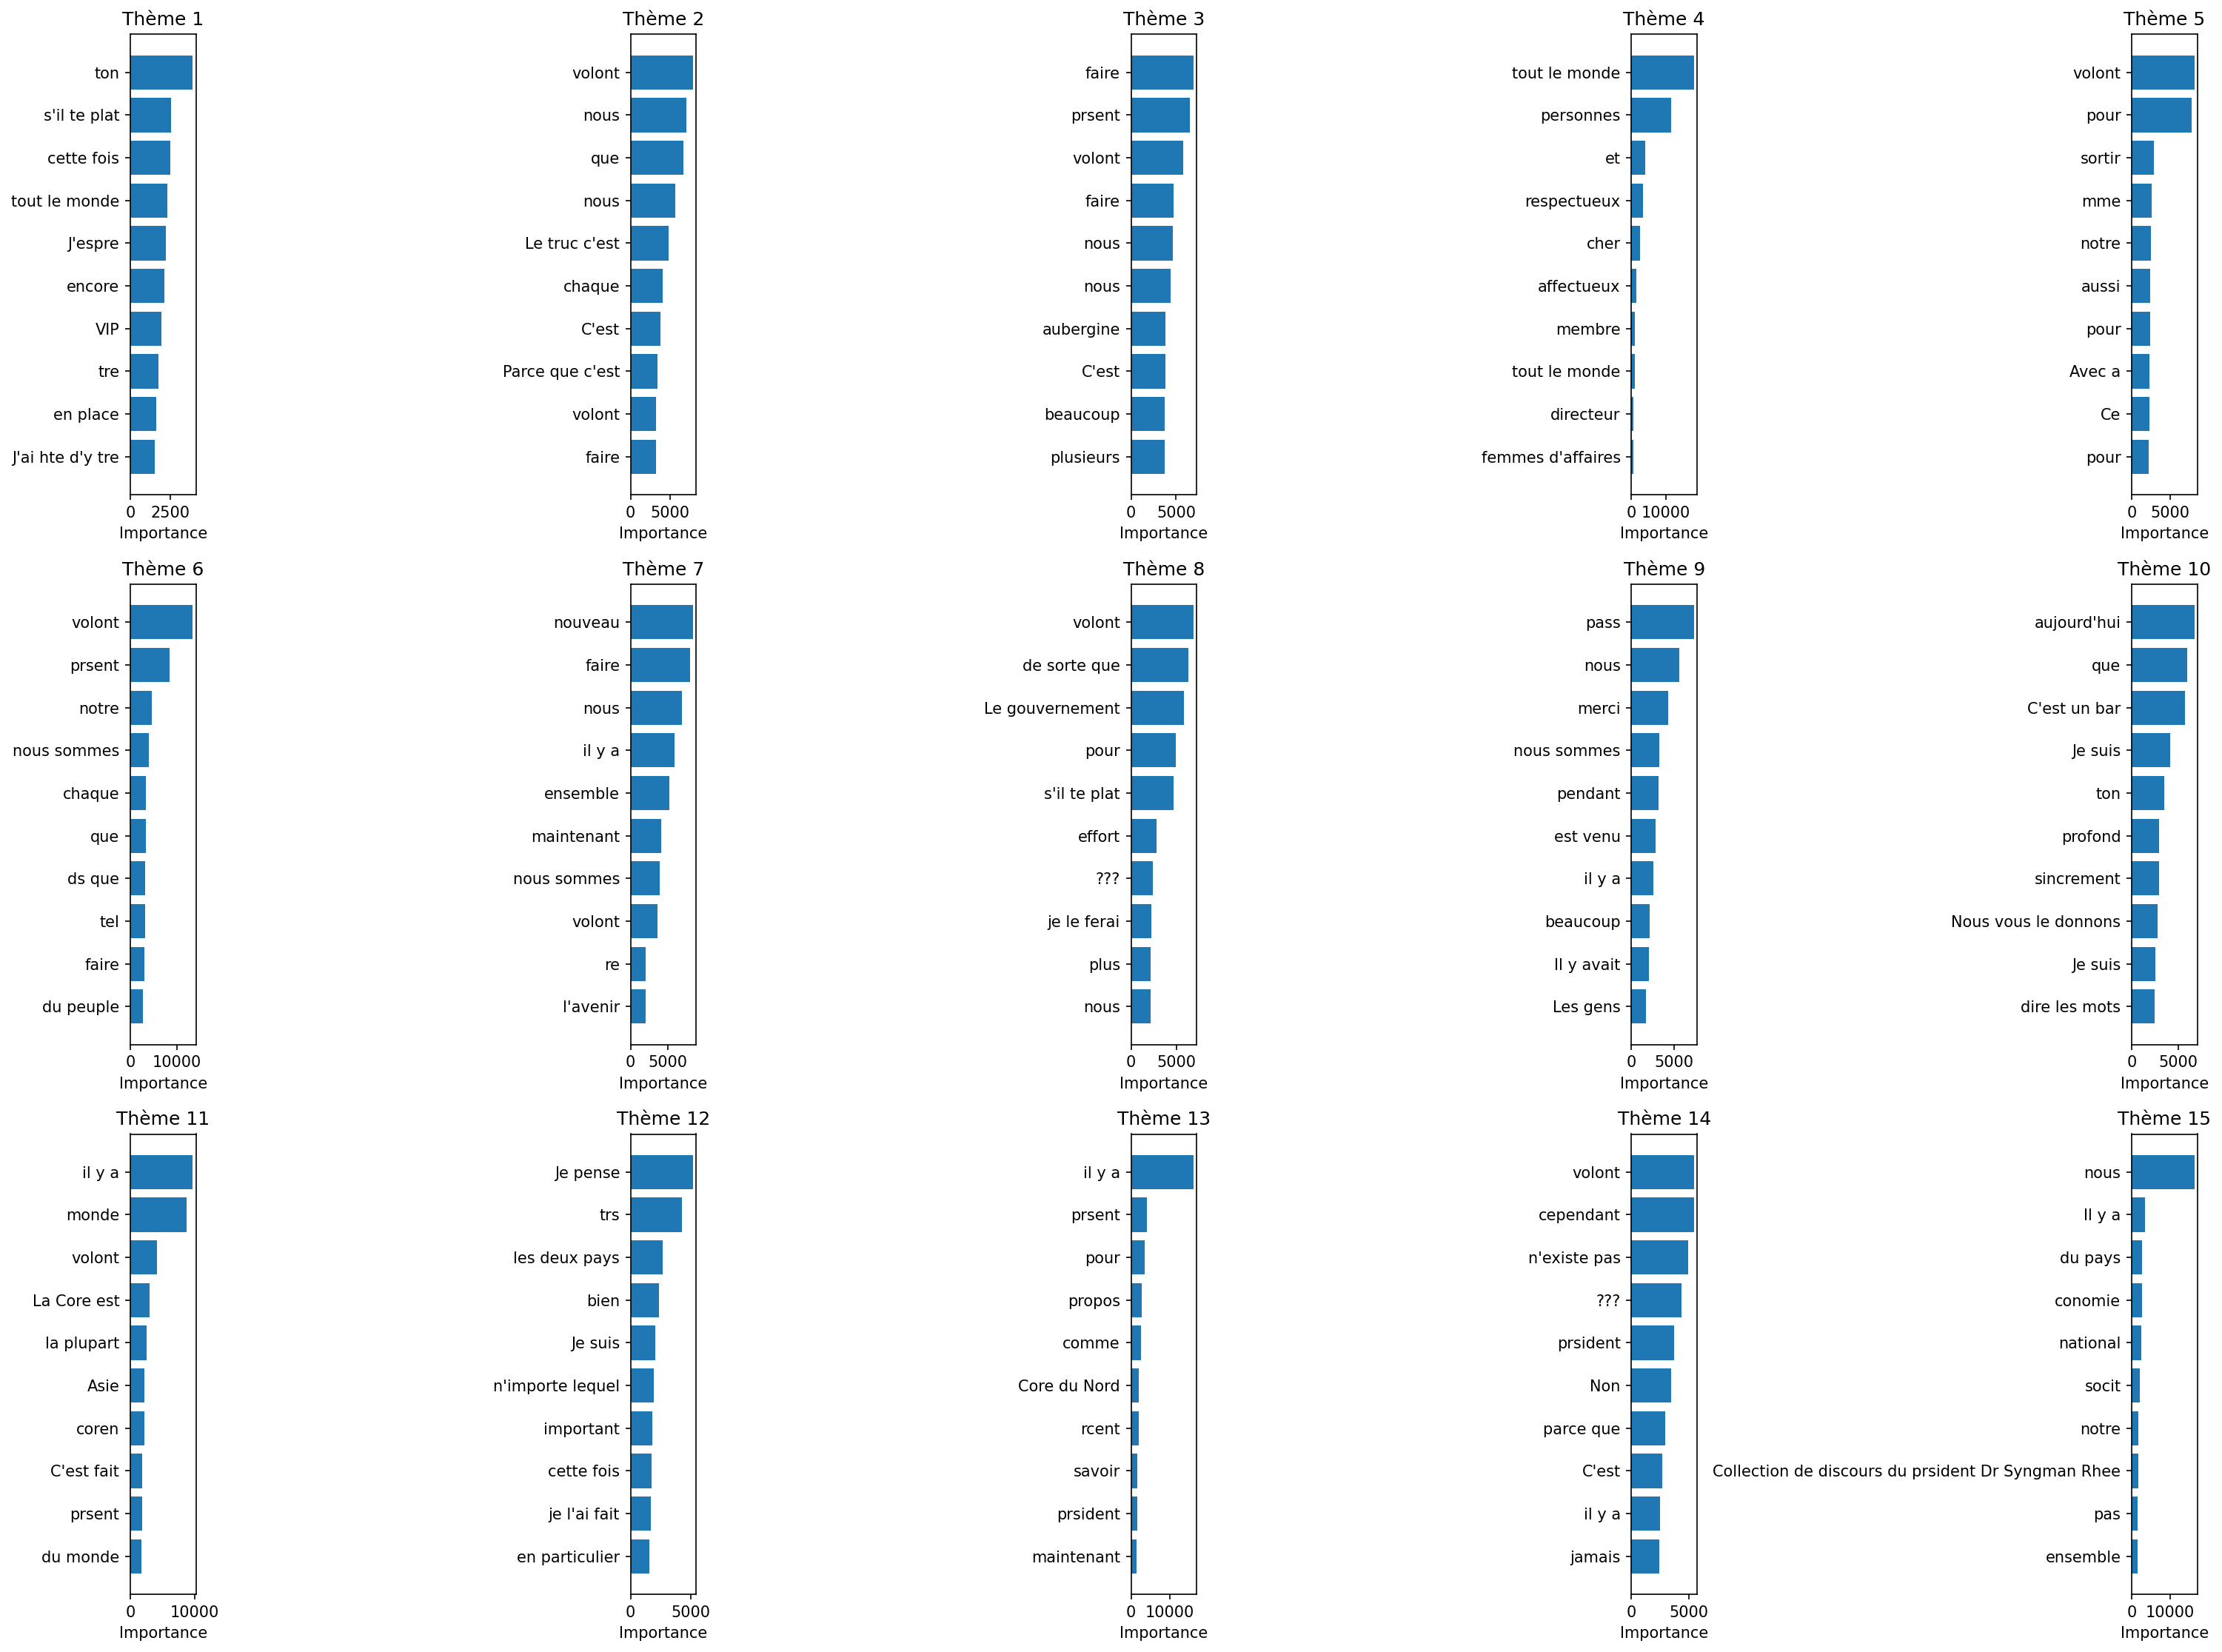
\includegraphics[width=0.8\textwidth]{lda_topics.png}
    \caption{Distribution des thèmes extraits par le modèle LDA (15 thèmes).}
    \label{fig:lda}
\end{figure}

\begin{figure}[h]
    \centering
    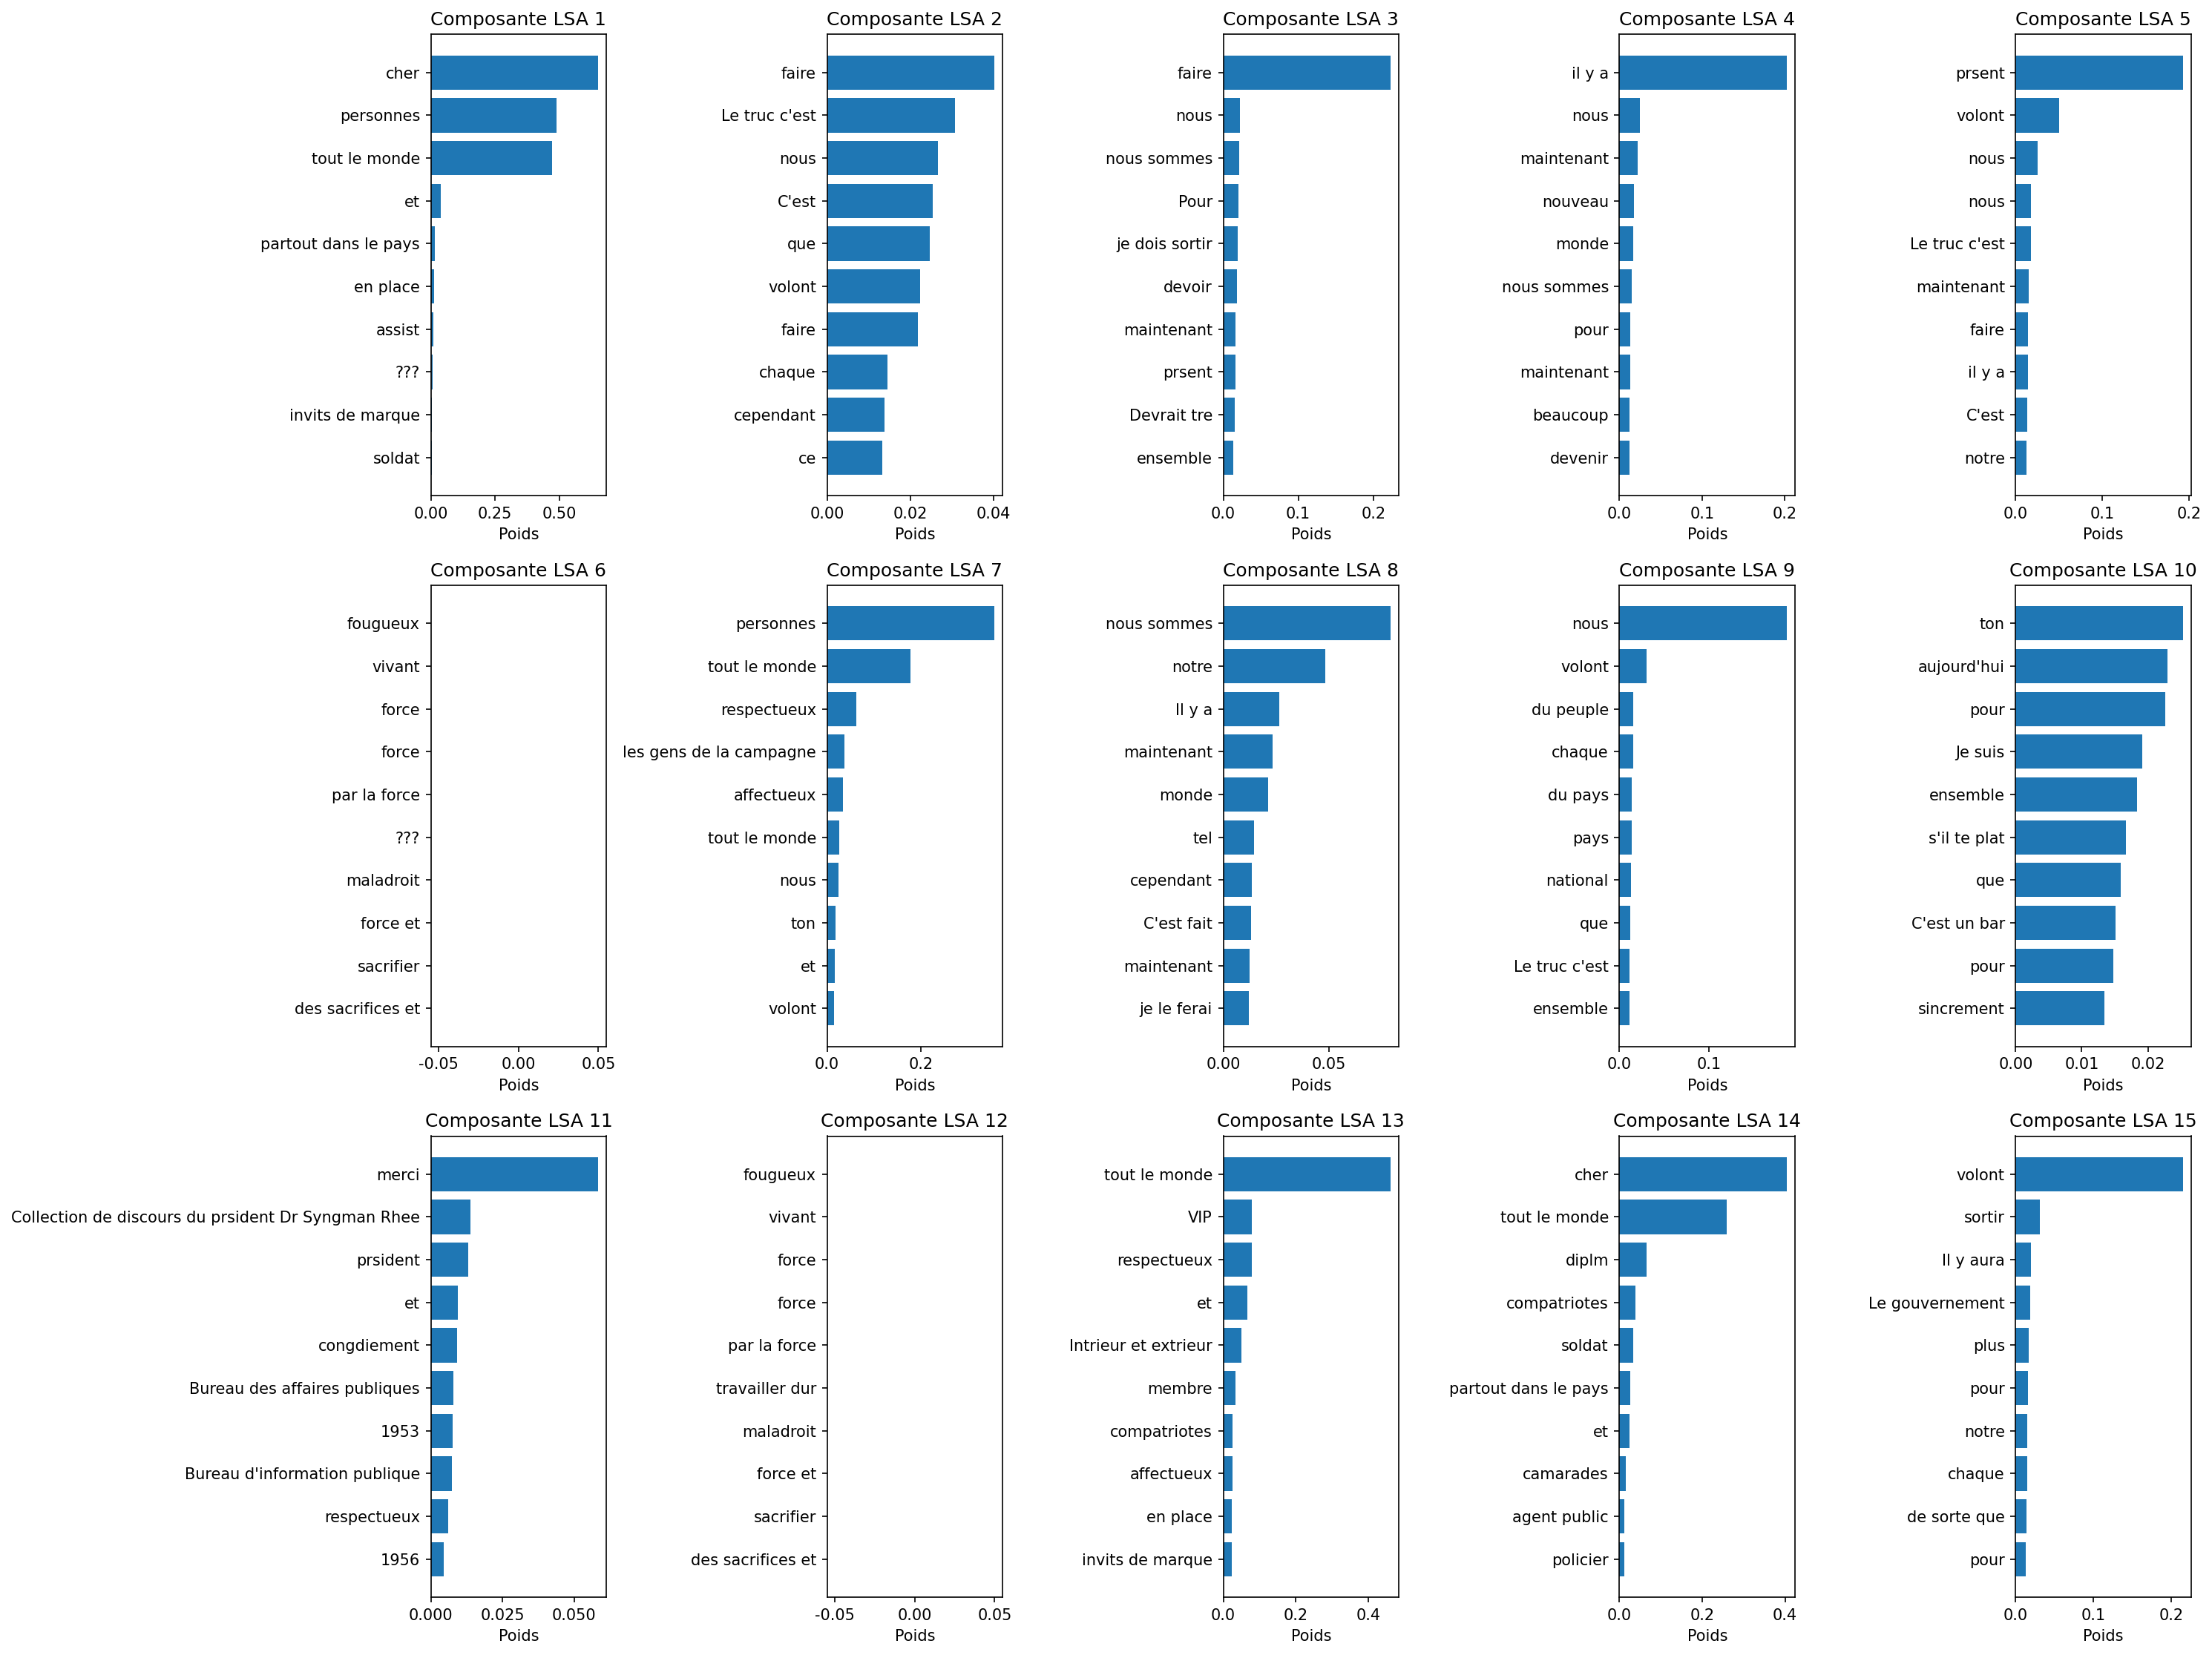
\includegraphics[width=0.8\textwidth]{lsa_components.png}
    \caption{Projection des composantes sémantiques via LSA.}
    \label{fig:lsa}
\end{figure}

\begin{figure}[h]
    \centering
    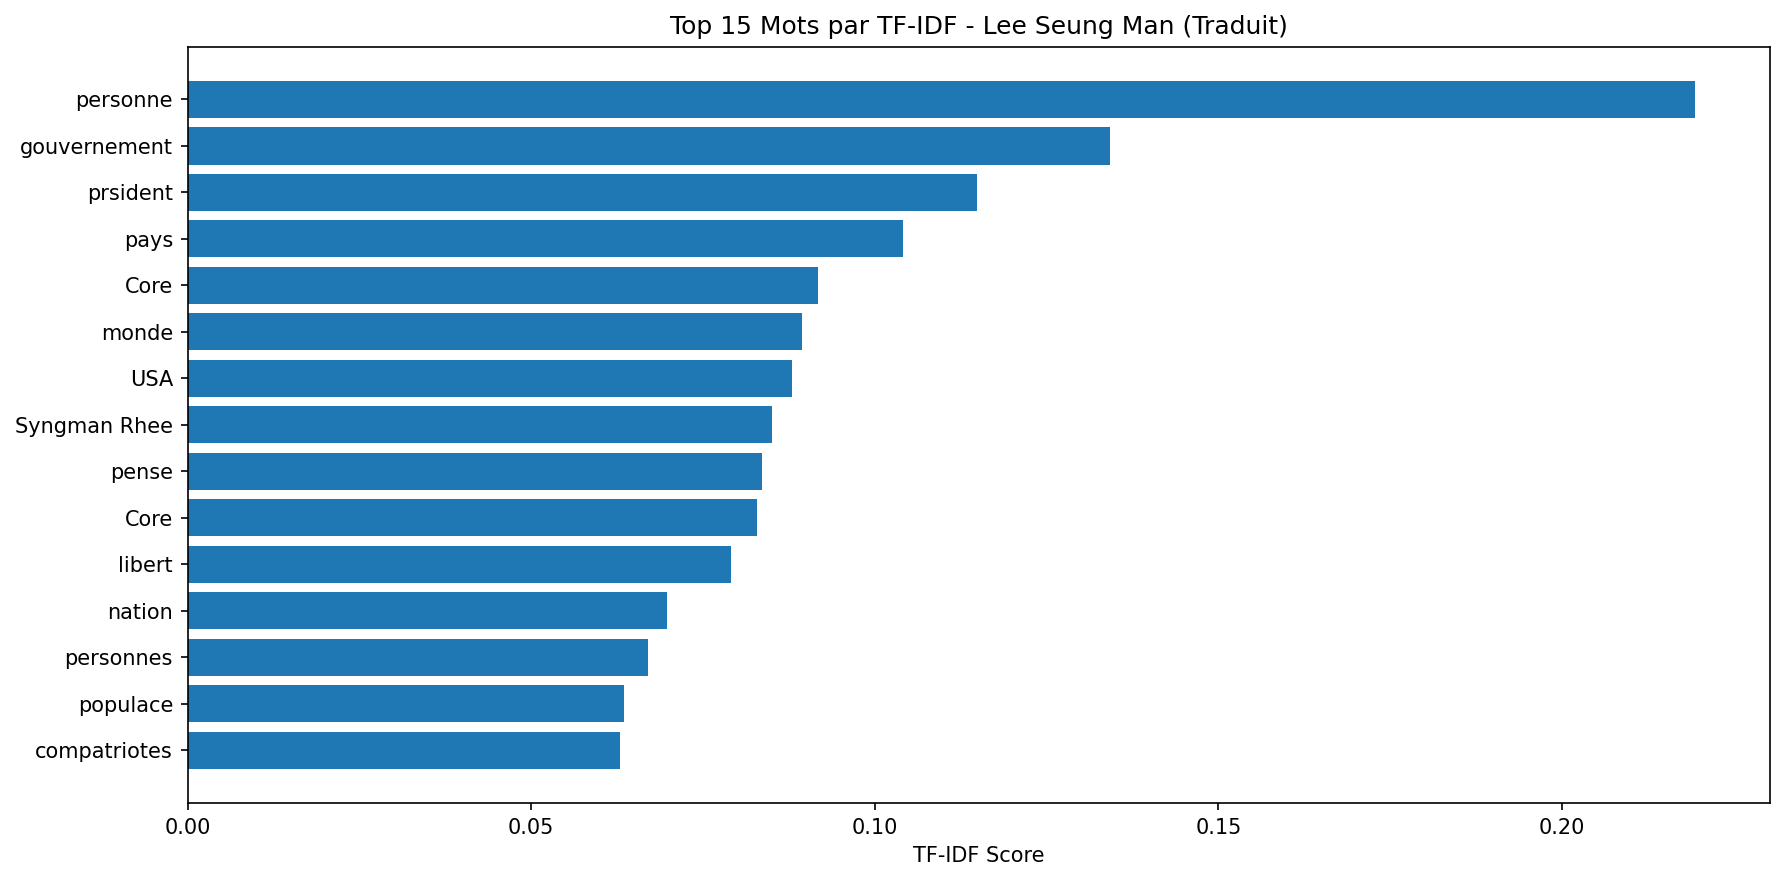
\includegraphics[width=0.8\textwidth]{tfidf_analysis.png}
    \caption{Analyse TF-IDF des termes les plus discriminants.}
    \label{fig:tfidf}
\end{figure}

\end{document}
